\documentclass[../main-sheet.tex]{subfiles}
\usepackage{../style}
\graphicspath{ {../img/} }
\backgroundsetup{contents={}}
\begin{document}
\chapter{Partial Differential Equations}
We consider the general second order partial Differential equation of the form
\begin{equation}
    A\frac{\partial^2 u}{\partial x^2}+B\frac{\partial^2 u}{\partial x\partial y}+C\frac{\partial^2 u}{\partial y^2}-F(x,y,u,\frac{\partial u}{\partial x},\frac{\partial u}{\partial y})=0 \label{eq:11pd1}
\end{equation}
If \(A\), \(B\) and \(C\) are functions of \(x\), \(y\), \(u\), \(\frac{\partial u}{\partial x}\) and \(\frac{\partial u}{\partial y}\). Then \eqref{eq:11pd1} is called a quasi linear PDE. When \(A\), \(B\) and \(C\) are functions of \(x\), \(y\) only and \(F\) is a linear function of \(u\), \(\frac{\partial u}{\partial x}\), \(\frac{\partial u}{\partial y}\). Then \eqref{eq:11pd1} is called linear PDE. A linear PDE may be written as 
\begin{equation}
    A\frac{\partial^2 u}{\partial x^2}+2B\frac{\partial^2 u}{\partial x\partial y}+C\frac{\partial^2 u}{\partial y^2}+D\frac{\partial u}{\partial x}+E\frac{\partial u}{\partial y}+Fu+G=0 \label{eq:11pd2}
\end{equation}
Where \(A\), \(B\), \(C\), \(D\), \(E\), \(F\) and \(G\) are constants or functions of \(x\) and \(y\) only. The equation \eqref{eq:11pd2} is homogeneous if \(G=0\); otherwise inhomogeneous.
\section{Introduction}
The general 2nd-order linear partial differential equation is of the form
\begin{align}
    &A\frac{\partial^2 u}{\partial x^2}+B\frac{\partial^2 u}{\partial x\partial y}+C\frac{\partial^2 u}{\partial y^2}+D\frac{\partial u}{\partial x}+E\frac{\partial u}{\partial y}+Fu=G\notag\\
    \text{or, }&Au_{xx}+Bu_{xy}+Cu_{yy}+Du_x+Eu_y+Fu=G\label{eq:11pd1.1}
\end{align}
where \(A\), \(B\), \(C\), \(D\), \(E\), \(F\) and \(G\) are constants or functions of \(x\) and \(y\) only.

Equation \eqref{eq:11pd1.1} can be classified with respect to the sign of the discreminant
\begin{equation}
    \Delta_s=B^2-4AC \label{eq:11pd1.2} 
\end{equation}
in the following way:
\begin{enumerate}[label=(\roman*)]
    \item If \(\Delta_s<0\) at a point in the \((x,y)\) plane the equation is said to be of elliptic type.
    \item Hyperbolic type when \(\Delta_s>0\) at the point in \((x,y)\) plane 
    \item Parabolic type when \(\Delta_s=0\) at the point in \((x,y)\) plane 
\end{enumerate}
Three simple particular cases of the equation \eqref{eq:11pd1.1} are
\begin{enumerate}[label=(\roman*)]
    \item Laplace equation: \(u_{xx}+u_{yy}=0\)
    \item Wave equation: \(u_{xx}-\frac{1}{c^2}u_{tt}=0\)
    \item Wave equation: \(u_{xx}-u_{t}=0\)
\end{enumerate}
where \((x,y)\) are space coordinates and \(t\) is the time coordinate. It is clear that Laplace equation is of elliptic type, that the wave equation is of hyperbolic type and the that the heat equation is of parabolic type.
\section{Finite Difference Approximations to Derivatives}
Let the \((x,y)\) plane be divided into a network of rectangles of sides \(\Delta x=h\) and \(\Delta y=k\) by drawing the sets of lines
\begin{align*}
    x&=ih;\qquad i=0,1,2,3,\dots\\
    y&=jk;\qquad j=0,1,2,3,\dots
\end{align*}
The points of intersection of these families of lines are called mesh points, lattice points or grid points. Then we have
\begin{align}
    u_x&=\frac{u_{i+1,j}-u_{i,j}}{h}+O(h)\label{eq:pde6}\\
    &=\frac{u_{i,j}-u_{i-1,j}}{h}+O(h)\label{eq:pde7}\\
    &=\frac{u_{i+1,j}-u_{i-1,j}}{2h}+O(h^2)\label{eq:pde8}\\
    \intertext{and }
    u_{xx}&=\frac{u_{i-1,j}-2u_{i,j}+u_{i+1,j}}{h^2}+O(h^2)\label{eq:pde9}
\end{align}
where \(u_{i,j}=u(ih,jk)=u(x,y)\). Similarly, we have the approximations
\begin{align}
    u_y&=\frac{u_{i,j+1}-u_{i,j}}{k}+O(k)\label{eq:pde10}\\
    &=\frac{u_{i,j}-u_{i,j-1}}{k}+O(k)\label{eq:pde11}\\
    &=\frac{u_{i,j+1}-u_{i,j-1}}{2k}+O(k^2)\label{eq:pde12}\\
    \intertext{and }
    u_{yy}&=\frac{u_{i,j-1}-2u_{i,j}+u_{i,j+1}}{k^2}+O(k^2)\label{eq:pde13}
\end{align}
The Laplace equation in two dimension is 
\[u_{xx}+u_{yy}=0\]
The finite difference analogue of this equation is
\begin{equation}
    \frac{1}{h^2}[u_{i+1,j}-2u_{i,j}+u_{i-1,j}]+\frac{1}{k^2}[u_{i,j+1}-2u_{i,j}+u_{i,j-1}]=0\label{eq:pde14}
\end{equation}
If \(h=k\) this gives
\begin{equation}
    u_{i,j}=\frac{1}{4}[u_{i+1,j}+u_{i-1,j}+u_{i,j+1}+u_{i,j-1}]\label{eq:pde15}
\end{equation}
Which shows that the value of \(u\) at any point is the mean of its value at the four neighboring points. This is called standard five-point formula (see fig 1(a)),
\begin{center}
    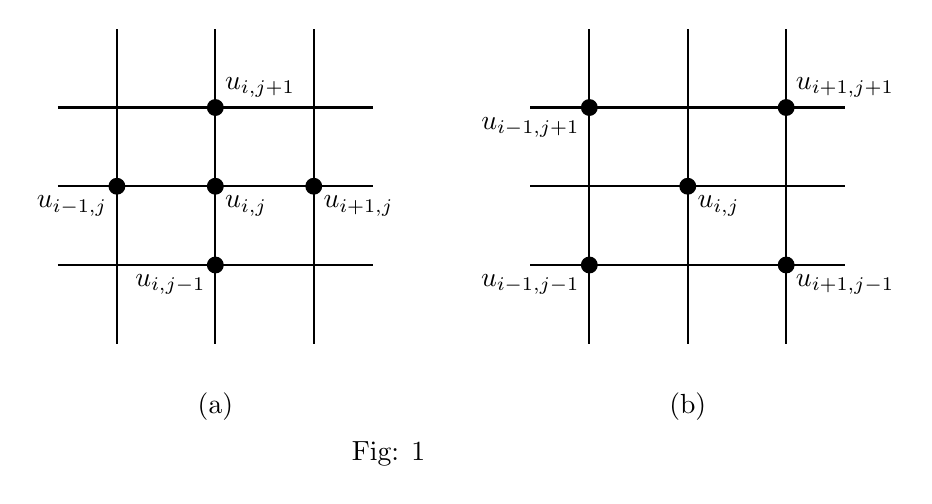
\begin{tikzpicture}
        \draw[thick] (-2,0)--(2,0);
        \draw[thick] (-2,-1)--(2,-1);
        \draw[thick] (-2,1)--(2,1);
        
        \draw[thick] (0,-2)--(0,2);
        \draw[thick] (1.25,-2)--(1.25,2);
        \draw[thick] (-1.25,-2)--(-1.25,2);
        \draw[fill=black] (0,0) circle (0.1)node[below right] {$u_{i,j}$};
        \draw[fill=black] (0,-1) circle (0.1)node[below left] {$u_{i,j-1}$};
        \draw[fill=black] (0,1) circle (0.1)node[above right] {$u_{i,j+1}$};
        \draw[fill=black] (-1.25,0) circle (0.1)node[below left] {$u_{i-1,j}$};
        \draw[fill=black] (1.25,0) circle (0.1)node[below right] {$u_{i+1,j}$};
        \node at (0,-2.8) {(a)};
        
        \node at (2.2,-3.4) {Fig: 1};
        \begin{scope}[xshift=6cm]
        \draw[thick] (-2,0)--(2,0);
        \draw[thick] (-2,-1)--(2,-1);
        \draw[thick] (-2,1)--(2,1);
        
        \draw[thick] (0,-2)--(0,2);
        \draw[thick] (1.25,-2)--(1.25,2);
        \draw[thick] (-1.25,-2)--(-1.25,2);
        \draw[fill=black] (0,0) circle (0.1)node[below right] {$u_{i,j}$};
        \draw[fill=black] (-1.25,-1) circle (0.1)node[below left] {$u_{i-1,j-1}$};
        \draw[fill=black] (1.25,1) circle (0.1)node[above right] {$u_{i+1,j+1}$};
        \draw[fill=black] (-1.25,1) circle (0.1)node[below left] {$u_{i-1,j+1}$};
        \draw[fill=black] (1.25,-1) circle (0.1)node[below right] {$u_{i+1,j-1}$};
        \node at (0,-2.8) {(b)};
        \end{scope}
        \end{tikzpicture}
\end{center}
and is written as
\begin{equation}
    u_{i+1,j}+u_{i-1,j}+u_{i,j+1}+u_{i,j-1}-4u_{i,j}=0\label{eq:pde16}   
\end{equation}
By expanding the terms on the RHS of \eqref{eq:pde15} by Taylor's series, it can be shown that,
\begin{equation}
    u_{i+1,j}+u_{i-1,j}+u_{i,j}+u_{i,j-1}-4u_{i,j}=h^2(u_{xx}+u_{yy})-\frac{1}{6}h^4 u_{xxyy}+O(h^6)=-\frac{1}{6}h^4 u_{xxyy}+O(h^6) \label{eq:pde17}
\end{equation}
Instead of \eqref{eq:pde15}, we may also use the formula
\begin{equation}
    u_{i,j}=\frac{1}{4}[u_{i-1,j-1}+u_{i+1,j-1}+u_{i+1,j+1}+u_{i-1,j+1}] \label{eq:pde18}
\end{equation}
which uses the function values at the diagonal points (fig-1(b)) and is therefore called the diagonal five point formulae.
\begin{ex}
    We wish to solve Laplace equation \(u_{xx}+u_{yy}=0\) in a bounded region \(R\) with boundary \(C\). Let the value of \(u\) be specified everywhere on \(C\). For simplicity, let \(R\) be a square region so that \(u\) can be divided into a network of small squares of side \(h\). Let the values of \(u(x,y)\) on the boundary \(C\) be given \(c_i\) and let the interior mesh points and the boundary points be as in fig-2.
    \begin{center}
        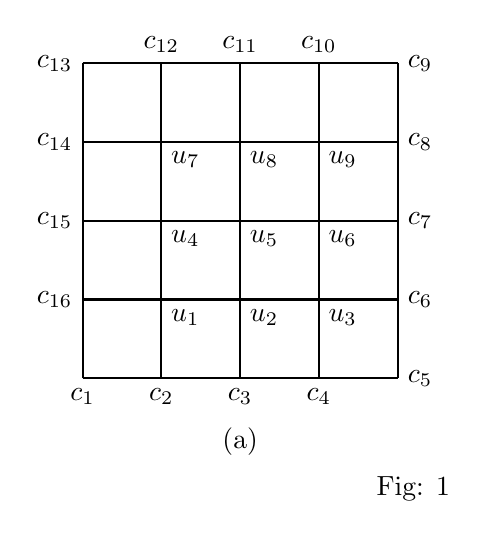
\begin{tikzpicture}
            \draw[thick] (-2,0)node[left] {$c_{15}$}--(2,0)node[right] {$c_7$};
            \draw[thick] (-2,-1)node[left] {$c_{16}$}--(2,-1)node[right] {$c_6$};
            \draw[thick] (-2,1)node[left] {$c_{14}$}--(2,1)node[right] {$c_8$};
            \draw[thick] (-2,2)node[left] {$c_{13}$}--(2,2)node[right] {$c_9$};
            \draw[thick] (-2,-2)--(2,-2)node[right] {$c_5$};
            
            \draw[thick] (0,-2)node[below] {$c_{3}$}--(0,2)node[above] {$c_{11}$};
            \draw[thick] (1,-2)node[below] {$c_{4}$}--(1,2)node[above] {$c_{10}$};
            \draw[thick] (-1,-2)node[below] {$c_{2}$}--(-1,2)node[above] {$c_{12}$};
            \draw[thick] (-2,-2)node[below] {$c_{1}$}--(-2,2);
            \draw[thick] (2,-2)--(2,2);
            \draw[fill=black] (0,0) circle (0)node[below right] {$u_{5}$};
            \draw[fill=black] (0,-1) circle (0)node[below right] {$u_{2}$};
            \draw[fill=black] (0,1) circle (0)node[below right] {$u_{8}$};
            \draw[fill=black] (-1,0) circle (0)node[below right] {$u_{4}$};
            \draw[fill=black] (1,0) circle (0)node[below right] {$u_{6}$};
            \draw[fill=black] (-1,-1) circle (0)node[below right] {$u_{1}$};
            \draw[fill=black] (-1,1) circle (0)node[below right] {$u_{7}$};
            \draw[fill=black] (1,1) circle (0)node[below right] {$u_{9}$};
            \draw[fill=black] (1,-1) circle (0)node[below right] {$u_{3}$};
            \node at (0,-2.8) {(a)};
            
            \node at (2.2,-3.4) {Fig: 1};
            
        \end{tikzpicture}
    \end{center}
    We can apply either standard five-point or diagonal five-point formula. The approximate function values at the interior mesh points can now be computed according to the scheme; we first use the diagonal five-point formula and compute \(u_5\), \(u_7\), \(u_9\), \(u_1\) and \(u_3\) in this order.

    Thus, we obtain
    \begin{align*}
        u_5&=\frac{1}{4}(c_1+c_5+c_9+c_{13})\\
        u_7&=\frac{1}{4}(c_{15}+u_5+c_{11}+c_{13})\\
        u_9&=\frac{1}{4}(u_{5}+c_7+c_{9}+c_{11})\\
        u_1&=\frac{1}{4}(c_{1}+c_3+u_{5}+c_{14})\\
        u_3&=\frac{1}{4}(c_{3}+c_5+c_{7}+u_{5})
    \end{align*}
    We then compute, the remaining quantities \(u_8\), \(u_4\), \(u_6\) and \(u_2\) by the standard five-point formula. We have,
    \begin{align*}
        u_8&=\frac{1}{4}(u_5+u_9+c_{11}+u_{7})\\
        u_4&=\frac{1}{4}(u_{1}+u_5+u_{7}+c_{15})\\
        u_6&=\frac{1}{4}(u_{5}+c_7+c_{9}+u_{5})\\
        u_2&=\frac{1}{4}(c_{3}+u_3+u_{5}+u_{1})
    \end{align*}
    when once all the \(u_i\) \((i=1,2,...,9)\) are computed, their accuracy can be improved by any of the iterative methods.\\
    \underline{Jacobi's Method:} Let \(u_{i,j}^{(n)}\) denote the \(n\)th iterative of \(u_{i,j}\). An iterative procedure to solve \eqref{eq:pde16} is
    \begin{equation}
        u_{i,j}^{(n+1)}=\frac{1}{4}\left[ u_{i-1,j}^{(n)}+u_{i+1,j}^{(n)}+u_{i,j-1}^{(n)}+u_{i,j+1}^{(n)} \right] \label{eq:pde19}
    \end{equation}
    for the interior mesh points. This is called the point Jacobi method.\\
    \underline{Gauss-Seidel Method:}
    \begin{equation}
        u_{i,j}^{(n+1)}=\frac{1}{4}\left[ u_{i-1,j}^{(n+1)}+u_{i+1,j}^{(n)}+u_{i,j-1}^{(n+1)}+u_{i,j+1}^{(n)} \right] \label{eq:pde20}
    \end{equation}
    \underline{SOR Method:}
    \begin{equation}
        u_{i,j}^{(n+1)}=\frac{1}{4}\omega \left[ u_{i-1,j}^{(n+1)}+u_{i+1,j}^{(n)}+u_{i,j-1}^{(n+1)}+u_{i,j+1}^{(n)} \right]+(1-\omega)u_{i,j}^{(n)} \label{eq:pde21}
    \end{equation}
\end{ex}
\begin{ex}
    Solve Laplace's equation for the square region shown in the following figure.
    \begin{center}
        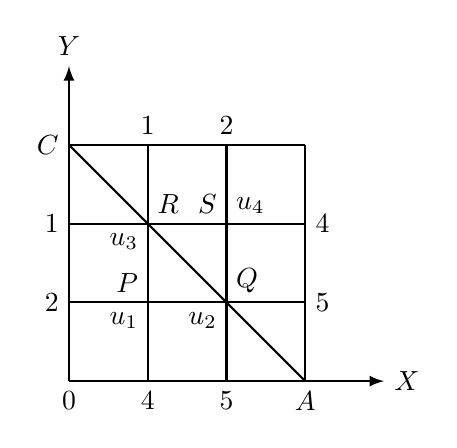
\begin{tikzpicture}
            \draw[thick] (-2,0)node[left] {$1$}--(1,0)node[right] {$4$};
            \draw[thick] (-2,-1)node[left] {$2$}--(1,-1)node[right] {$5$};
            \draw[thick] (-2,1)node[left] {$C$}--(1,1);
            % \draw[thick] (-2,2)node[left] {$c_{13}$}--(2,2)node[right] {$c_9$};
            \draw[thick,-latex] (-2,-2)--(2,-2)node[right] {$X$};
            
            \draw[thick] (0,-2)node[below] {$5$}--(0,1)node[above] {$2$};
            \draw[thick] (1,-2)node[below] {$A$}--(1,1);
            \draw[thick] (-1,-2)node[below] {$4$}--(-1,1)node[above] {$1$};
            \draw[thick,-latex] (-2,-2)node[below] {$0$}--(-2,2)node[above] {$Y$};
            % \draw[thick] (2,-2)--(2,2);
            \draw[fill=black] (0,0) circle (0)node[above right] {$u_{4}$}node[above left] {$S$};
            \draw[fill=black] (0,-1) circle (0)node[below left] {$u_{2}$}node[above right] {$Q$};
            % \draw[fill=black] (0,1) circle (0)node[below right] {$u_{8}$};
            \draw[fill=black] (-1,0) circle (0)node[below left] {$u_{3}$}node[above right] {$R$};
            % \draw[fill=black] (1,0) circle (0)node[below right] {$u_{6}$};
            \draw[fill=black] (-1,-1) circle (0)node[below left] {$u_{1}$}node[above left] {$P$};
            \draw[thick] (-2,1)--(1,-2);
            \end{tikzpicture}
    \end{center}
\end{ex}
\begin{soln}
    From the figure we observe that the boundary values are symmetric about the diagonal \(AC\). Hence, \(u_1=u_4\). So we need to find only \(u_1\), \(u_2\) and \(u_3\).\\
    Standard five-point formula is
    \begin{equation}
        u_{i,j}=\frac{1}{4}(u_{i+1,j}+u_{i-1},j+u_{i,j+1}+u_{i,j-1})
        \label{eq:pdep1.1}
    \end{equation}
    At \(p\) we have from \eqref{eq:pdep1.1}
    \begin{equation}
        u_1=\frac{1}{4}(u_2+u_3+2+4)=\frac{1}{4}(u_2+u_3+6)\label{eq:pdep1.2}
    \end{equation}
    At \(Q\),
    \begin{align}
        u_2&=\frac{1}{4}(u_1+u_4+5+5)\notag\\
        &=\frac{1}{4}(2u_1+10)\quad \because u_1=u_4\notag\\
        &=\frac{1}{2}(u_1+5)\label{eq:pdep1.3}
    \end{align}
    At \(R\)
    \begin{equation}
        u_3=\frac{1}{4}(u_2+1+u_4+1)=\frac{1}{2}(1+u_1)\label{eq:pdep1.4}
    \end{equation}
    Gauss-Seidel iterative form for \eqref{eq:pdep1.2}, \eqref{eq:pdep1.3} and \eqref{eq:pdep1.4} are as follows:
    \begin{align*}
        u_1^{(n+1)}&=\frac{1}{4}(u_2^{(n)}+u_3^{(n)}+6)\\
        u_2^{(n+1)}&=\frac{1}{4}(2u_1^{(n+1)}+10)\\
        u_3^{(n+1)}&=\frac{1}{4}(2u_1^{(n+1)}+2)
    \end{align*}
    1st iteration(\(n=0\)):\\
    (For 1st iteration, let \(u_2^{(0)}=5\), since it is near to the value 5 and \(u_3^{(0)}=1\) )
    \begin{align*}
        u_1^{(1)}&=\frac{1}{4}(u_2^{(0)}+u_3^{(0)}+6)\\
        &=\frac{1}{4}(5+1+6)\\
        &=3\\
        u_2^{(1)}&=\frac{1}{4}(2u_1^{(1)}+10)=\frac{1}{4}(2\times 3+10)=4\\
        u_3^{(1)}&=\frac{1}{4}(2u_1^{(1)}+2)=\frac{1}{4}(2\times 3+2)=2
    \end{align*}
    For \(n=1\):
    \begin{align*}
        u_1^{(2)}&=\frac{1}{4}(u_2^{(1)}+u_3^{(1)}+6)=\frac{1}{4}(4+2+6)=3\\
        u_2^{(2)}&=\frac{1}{4}(2u_1^{(2)}+10)=4\\
        u_3^{(2)}&=\frac{1}{4}(2u_1^{(2)}+2)=2
    \end{align*}
    Hence, \(u_1=3\), \(u_2=4\), \(u_3=2\), \(u_4=3\)
\end{soln}
\end{document}